\chapter{Analysis}

\section{Introduction}

\subsection{Client Identification}
my client is Susannah Mason, she is 50 years old and has very little usage of computers, except when having to order new stock for the pharmacy. currently the pharmacy uses computerised methods to submit orders to the warehouse.

Suesannah is a pharmacutical manager at spire healthcare in impington 

by  creating this program it would speed up the process making leeping track of and ordering of new equipment and stock alot easier for her 
\subsection{Define the current system}
 the current system uses mostly computer based order submission and price checks but the orders have to be put through the computer manually 
\subsection{Describe the problems}
the orders for the stock take too long to submit and all stock has to be conted by hand 
\subsection{Section appendix}

\section{Investigation}
\subsection{The current system}
the current system at the pharmacy is a data base that holds the information of over 500 items. the data base holds the price the mass the desription and how much is in the pharmacy at that point in time. when an item is taken out of stock the pharmacist has a card to say that an item has been removed from the storage cupboard. sometimes the system deosn't update even when the card is swiped to say a product has been removed
\subsubsection{Data sources and destinations}
\begin{table}[t]
\begin{tabular}{|c|c|c|}
\hline
Data Source & Travels via & destination\\
\hline
doctor & gives prescription & patient\\
\hline
patient & requests medicine & pharmacist\\
\hline
pharmacist & checks stock & stock system\\
\hline 
stock system & gives information & pharmasict\\
\hline
pharmacist & collects medication & medicine cupboard\\
\hline
pharmacist & gives medicine & patient
\hline
\end{tabular}
\caption{}
\label{tab:}
\end{table}
\subsubsection{Algorithms}

i will be using quite a few algorithums for this assignment

IF (item = lowest minimum amount) THEN
		order more item

ELSE
		check next item

END IF
\space
this other algorithm will be used to calculate the exact price of all of the order 

if order submitted = True THEN
		calculate order

ELSE 
		restart program

END IF
\space
using the information in the list Items the exact price is calulated

IF item in Items
		add price item

ELSE
		add price 0

END IF

\subsubsection{Data flow diagram}




\subsubsection{Input Forms, Output Forms, Report Formats}

\subsection{The proposed system}
the proposed system will be used to order, check stock and be informed as soon as anything leaves the pharmacy the data base will be updated of the removal, as well as if the product falls below a certain point it will be program to replace the stock by ordering new stock form the wearhouse automatically but the order will go through a master contol point before being sent off 
\subsubsection{Data sources and destinations}
\begin{table}
\begin{tabular}{|c|c|c|}
\hline\hline
data Source & travels via & destination\\
\hline
stock information & request for stock information & pharmacy computer\\
\hline
stock price & request stock price & pharmacy computer\\
\hline
show stock info & display info & pharmacist\\ 
\hline
\end{tabular}
\label{table:nonlin}

\end{table}
\subsubsection{Data flow diagram}

\subsubsection{Data dictionary}
\begin{table}
\begin{tabular}{|c|c|c|c|}
\hline
Data & Uses & Name \\
\hline

\end{tabular}
\label{table:nonlin}
\end{table}

\subsubsection{Volumetrics}

\section{Objectives}
\subsection{General Objectives}
\begin{itemize}
	\item to make a stable system that checks, updates, restocks and sends payment for the ordered items
	\item to give the system to auto restock items when they fall below a certain number of items
	\item to graph which items are being bought or used faster and updates the resocking system acordingly 
\end{itemize}
\subsection{Specific Objectives}
\begin{itemize}
	\item to design a program that will make sorting through the items at the pharmacy as well as store the price and item location in the pharmacy as well as the amount.
\end{itemize}
\subsection{Core Objectives}
\begin{itemize}
\item self updating stock system
\item easy accessablilty
\item order more items to refill stock
\end{itemize}
\subsection{Other Objectives}
\begin{itemize}
    \item the stock keeping on the program should be accurate. E.G. showing how much on tablet of paracitamol costs
    \item the system must have a automatic communication between the wholesale (warehouse) and the pharmacy
\end{itemize}
\section{ER Diagrams and Descriptions}
\subsection{ER Diagram}
\begin{figure}[ht!]
\centering
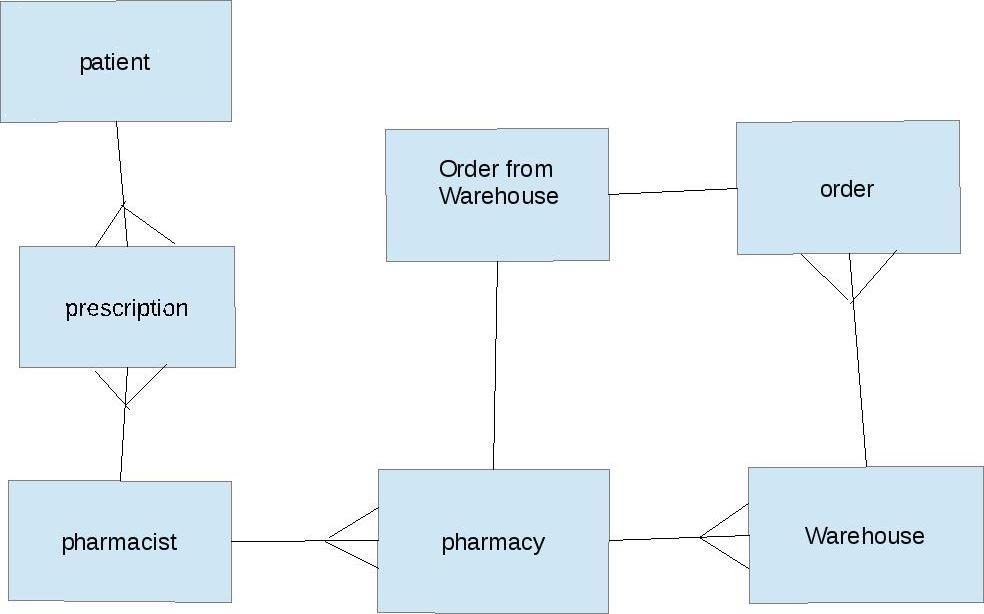
\includegraphics[width=90mm]{table 1.jpg}
\caption{A simple caption \label{overflow}}
\end{figure}
\subsection{Entity Descriptions}
\begin{itemize}
\item Client(\underline{clientID}, PharmacyNum, surname, FirstName, PhoneNumber, Address,Postcode)
\item Pharmacist(\underline{PharamacistID},\emph{PharmacyNum},Surname,FirstName,PhoneNumber,Address,Email)
\item Pharmacy(\underline{PharmacyNum},PharmacyAddress,PharmacyPhoneNumber)
\item Warehouse(\underline{WareHouseNum},\emph{PharmacyAddress},WareHouseAddress)
\item Order(\underline{OrderNum},\emph{WareHouseNum},\emph{PharmacyLocation},OrderDate,size)
\end{itemize}
\section{Object Analysis}

\subsection{Object Listing}
\begin{itemize}

\item Client
\item Pharmacist
\item Pharmacy
\item Warehouse
\item Order

\end{itemize}
\subsection{Relationship diagrams}

\subsection{Class definitions}

\section{Other Abstractions and Graphs}

\section{Constraints}

\subsection{Hardware}

\subsection{Software}

\subsection{Time}

\subsection{User Knowledge}

\subsection{Access restrictions}
the proposed system should only be accessable and privileges to the people in pharmacy, as well as the system should be password protectedto ensure no body outside the system can access the stock information.
\space

\section{Limitations}

\subsection{Areas which will not be included in computerisation}

\subsection{Areas considered for future computerisation}

\section{Solutions}
\subsection{Alternative solutions} 
\begin{table}
\begin{tabular}{|c|c|c|}
\hline
solution & advantages & disadvantages\\
\hline
problem & solved & hopwfully\\
\hline
\end{tabular}
\caption{}
\label{tab:nonlin}
\end{table}
\subsection{Justification of chosen solution}
I have chosen to the Python 3.2 desktop application with a GUI and SQL' solution. My reason for using this method is:
\begin{itemize}
    \item the application will be specific for pharmacy which will be updated at the start of every week and will continuously keep track of the database where the old system.
    \item the database used will take up less space required to store the data.
    \item due to the databases size making back ups is very easy so if the system.
\end{itemize} 
